\documentclass{standalone}

\usepackage{tikz}
\usetikzlibrary{calc}
\newcommand{\set}[1]{\left{ #1 \right}}

\begin{document}

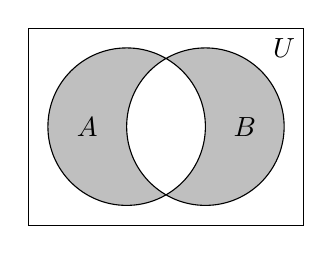
\begin{tikzpicture}
\draw (-1.25,-1.25) rectangle (2.25,1.25);
\fill[lightgray,even odd rule] (0,0) circle(1) (1,0) circle (1);
\draw[black] (0,0) circle (1) (1,0) circle (1);
\node at (-0.5,0) {$A$};
\node at (1.5,0) {$B$};
\node at (2,1) {$U$};
\end{tikzpicture}

\end{document}